\chapter{実験結果}
\section{ブロードコンタクトレーザーバー試料に関する測定結果}%=====================================
ブロードコンタクトレーザーバーに関してはウエハの特性を調べるために定常電流を流して測定を行なった。熱の発生を抑制するためにパルス電流を用いた。電流は...ms秒周期、...μsのパルス電流を流した。μs程度の電流は試料にとっては定常と見なされる。
まずは定常状態の測定。発振閾値電流を測定することに加えて、発振時の印可電流の増分したいする光出力の増大から発光量子効率を見積もることが目的である。
様々なパラメータを測定する。ウエハの構造ごとに節を分けている。
\subsection{3QW}%===============================
\begin{figure}[h]
	\centering
	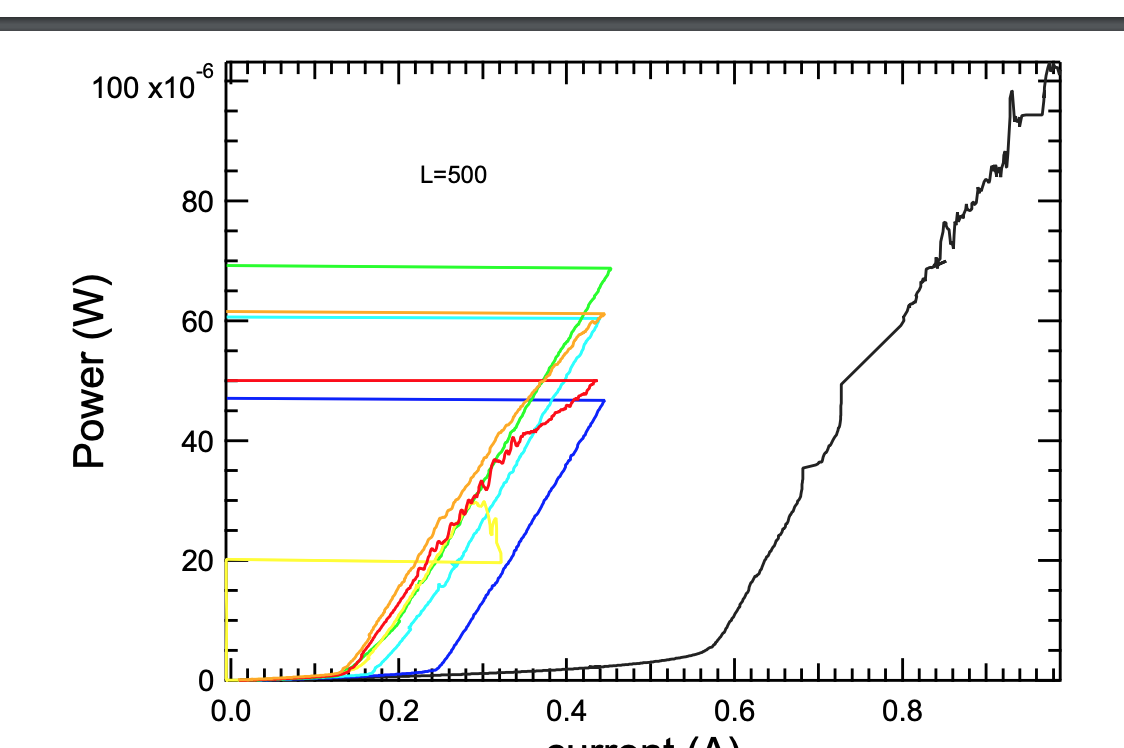
\includegraphics[width=10cm]{figure/fig_3_1_IL_broad_3QW.png}
		\caption{3MQWのIL結果}
		\label{fig_3_1_IL_3QW.png}
\end{figure}
閾値の表この表違うかも
\begin{table}[hbtp]
  \caption{閾値}
  \label{table:data_type}
  \centering
  \begin{tabular}{lcr}
    \hline
    共振器長  & 宣言  &  ビット幅  \\
    \hline \hline
    文字型  & char  & 8 \\
    整数型  & int   & 32 \\
    倍精度実数型  & double  & 64 \\
    倍々精度実数型  &  long double  &  96 \\
    \hline
  \end{tabular}
\end{table}

\begin{figure}[h]
	\centering
	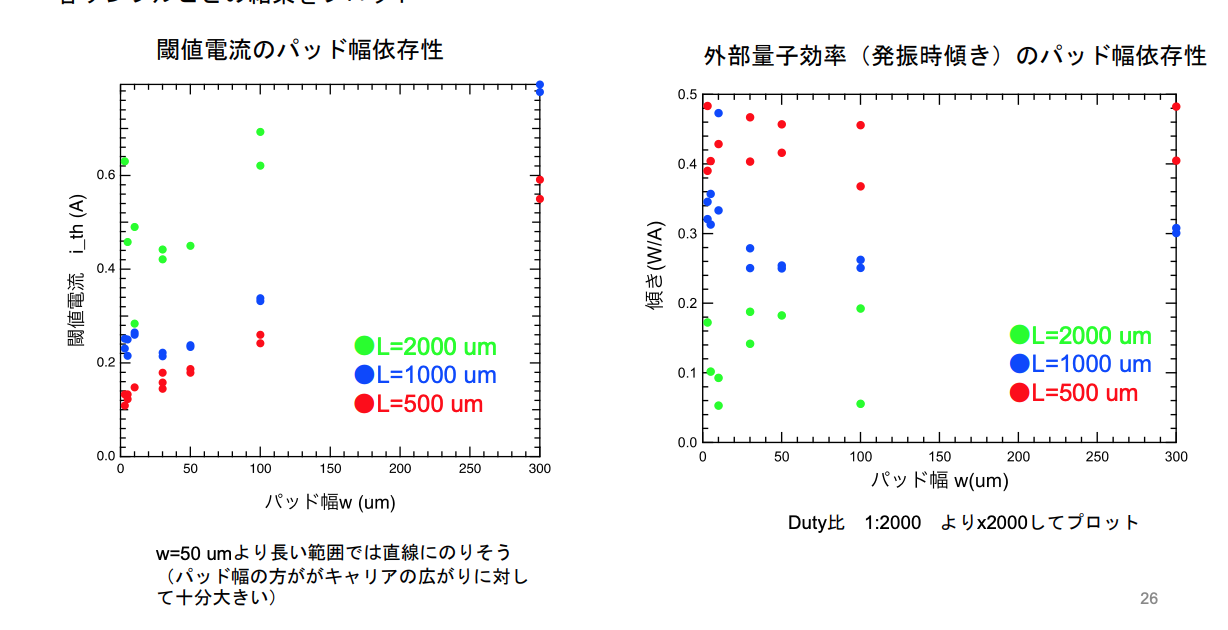
\includegraphics[width=10cm]{figure/fig_3_1_broad_i_th_3QW.png}
		\caption{3MQWの閾値電流}
		\label{fig_3_1_broad_i_th_3QW}
\end{figure}

\begin{figure}[h]
	\centering
	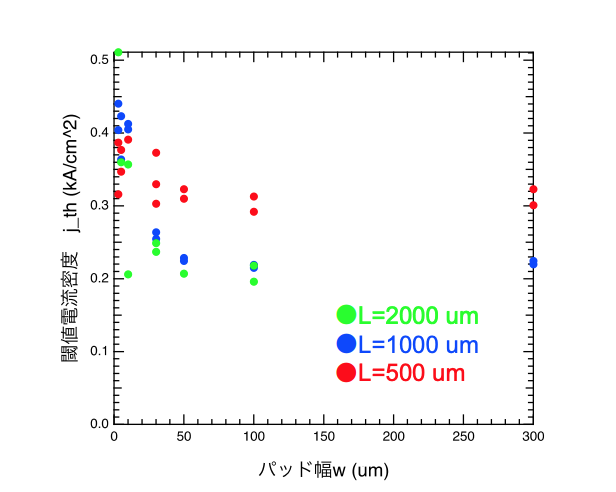
\includegraphics[width=10cm]{figure/fig_3_1_broad_j_th_3QW.png}
		\caption{3MQWの閾値電流密度のパッド幅依存性}
		\label{fig_3_1_broad_j_th_3QW}
\end{figure}

\newpage
\subsection{10QW}%===============================
\begin{figure}[h]
	\centering
	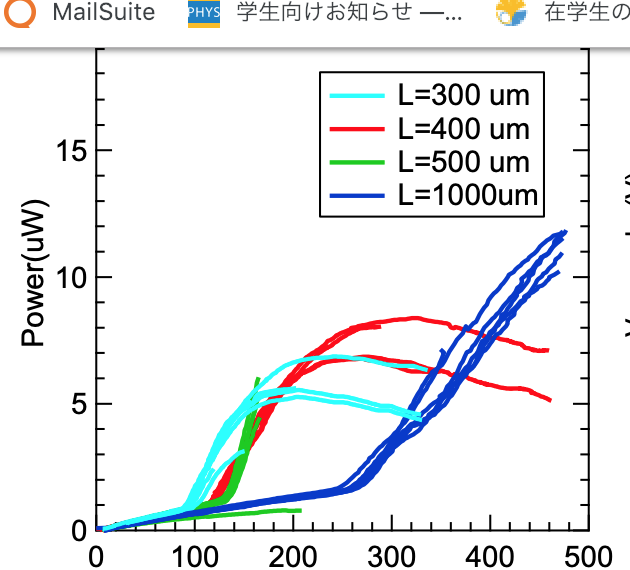
\includegraphics[width=10cm]{figure/fig_3_1_IL_10QW.png}
		\caption{10MQWのIL結果}
		\label{fig_3_1_IL_10QW.png}
\end{figure}
\begin{figure}[h]
	\centering
	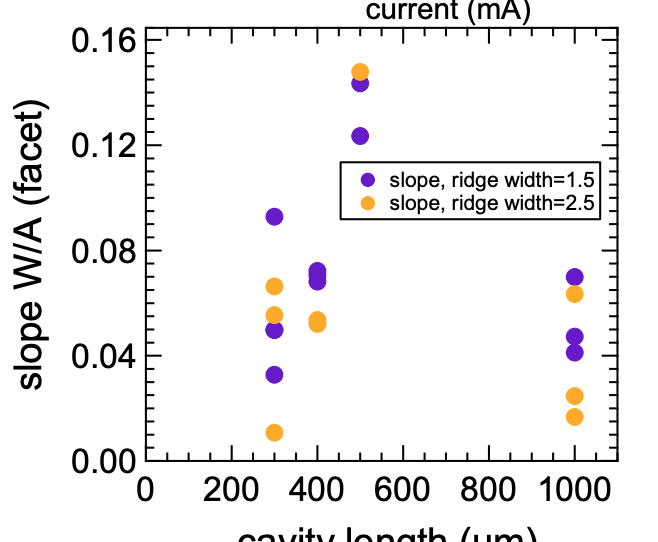
\includegraphics[width=10cm]{figure/fig_3_1_broad_slope_10QW.png}
		\caption{10MQWのスロープ}
		\label{fig_3_1_IL_broad_slope}
\end{figure}
閾値の表この表違うかも
\begin{table}[hbtp]
  \caption{閾値}
  \label{table:data_type}
  \centering
  \begin{tabular}{lcr}
    \hline
    共振器長  & 宣言  &  ビット幅  \\
    \hline \hline
    文字型  & char  & 8 \\
    整数型  & int   & 32 \\
    倍精度実数型  & double  & 64 \\
    倍々精度実数型  &  long double  &  96 \\
    \hline
  \end{tabular}
\end{table}

\begin{figure}[h]
	\centering
	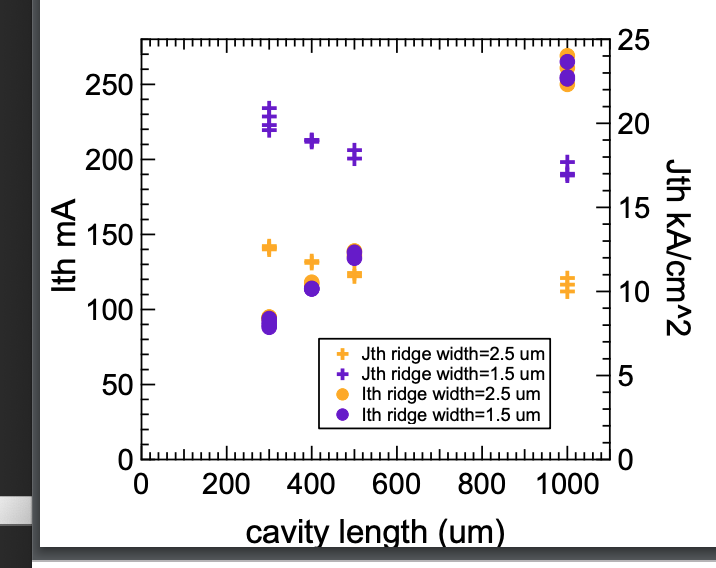
\includegraphics[width=10cm]{figure/fig_3_1_broad_i_th_10QW.png}
		\caption{10MQWの閾値電流}
		\label{fig_3_1_broad_i_th_3QW}
\end{figure}

\begin{figure}[h]
	\centering
	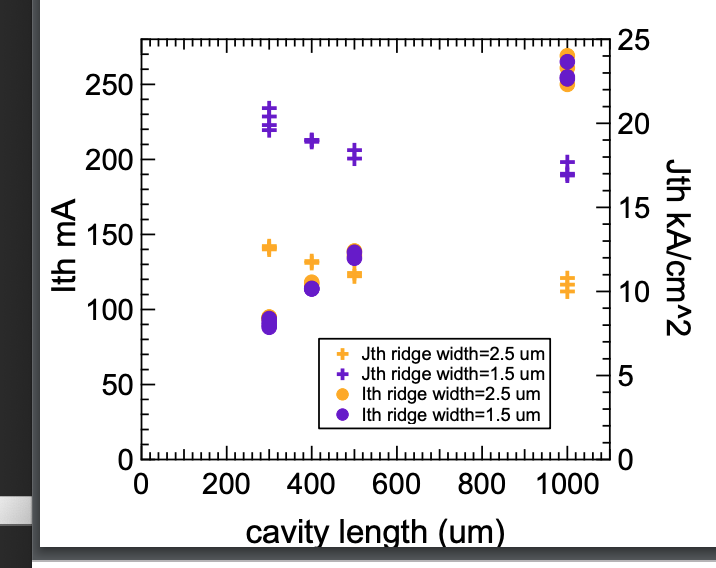
\includegraphics[width=10cm]{figure/fig_3_1_broad_i_th_10QW.png}
		\caption{10MQWの閾値電流密度のパッド幅依存性}
		\label{fig_3_1_broad_j_th_10QW}
\end{figure}

\newpage
\subsection{内部量子効率と吸収係数の計算}%=============
\begin{figure}[htbp]
	\centering
	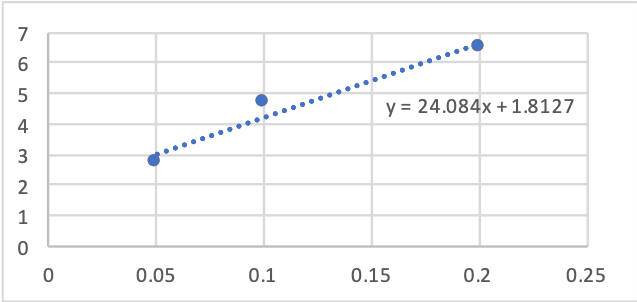
\includegraphics[width=10cm]{figure/fig_efficientcy_vs_L_inverce.png}
	\caption{外部量子効率 対共振器長の逆数}
	\label{fig:efficientcy_vs_L_inverce}
\end{figure}
\begin{figure}[h]
	\centering
	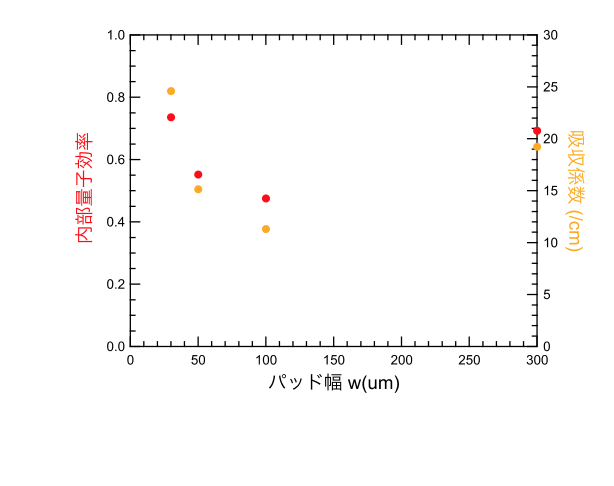
\includegraphics[width=10cm]{figure/fig_3_1_eff_in_3QW.png}
		\caption{3MQWのIL結果}
		\label{fig_3_1_IL_broad_i_th_3QW}
\end{figure}
\subsection{電流広がりに関する考察}%==================

\newpage
\newpage
\newpage
\section{電流注入利得スイッチング}%===================
リッジ導波路型レーザーに関して電流注入利得スイッチング実験を行った。その結果を示す。
\subsection{3QW}%===============================

\subsection{10QW}%==============================


